
\documentclass[../../../all/physics-standard_questions_all.tex]{subfiles}

\graphicspath{{../../../../figures/}}

\begin{document}

\begin{enumerate}

    \item 図のように，電池E（起電力$V_0$），電気抵抗$\mathrm{R}_1$（抵抗値$2R$），
        $\mathrm{R}_2$（抵抗値$3R$）からなる回路がある．AB間の合成抵抗$R_\mathrm{T}$を求めよ．
        \par \vspace{0.2\baselineskip}
        {\centering
            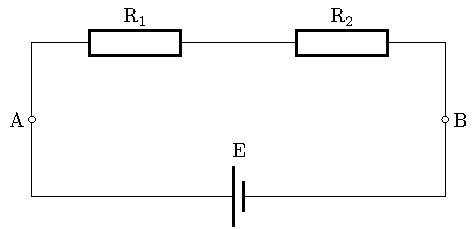
\includegraphics{q_circuit-extent_03_01/physics-standard_questions_circuit-extent_03_01_tikz.pdf}
        \par}
        \vspace{0.2\baselineskip}
    
    \item 図のように，電池E（起電力$V_0$），
        電気抵抗$\mathrm{R}_1$（抵抗値$2R$），$\mathrm{R}_2$（抵抗値$3R$）からなる回路がある．
        AB間の合成抵抗$R_\mathrm{T}$を求めよ．
        \par \vspace{0.2\baselineskip}
        {\centering
            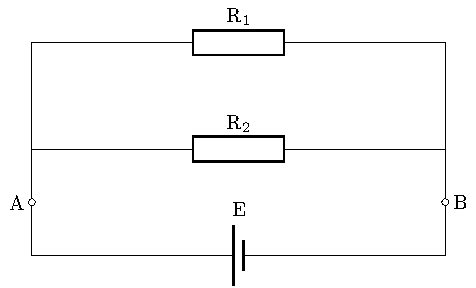
\includegraphics{q_circuit-extent_03_02/physics-standard_questions_circuit-extent_03_02_tikz.pdf}
        \par}
        \vspace{0.2\baselineskip}
    
    \item 図のように，電池E$_1$（起電力$2V_0$），E$_2$（起電力$V_0$），
    電気抵抗$\mathrm{R}_1$（抵抗値$2R$），$\mathrm{R}_2$（抵抗値$R$），$\mathrm{R}_3$（抵抗値$2R$）からなる回路がある．
    AB間の合成抵抗$R_\mathrm{T}$を求めよ．
        \par \vspace{0.2\baselineskip}
        {\centering
        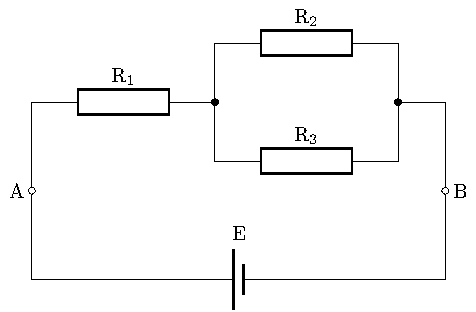
\includegraphics{q_circuit-extent_03_03/physics-standard_questions_circuit-extent_03_03_tikz.pdf}
        \par}
        \vspace{0.2\baselineskip}
    
    \item \needspace{8\baselineskip}
        図のように，電気抵抗$\mathrm{R}_1$，$\mathrm{R}_2$，$\mathrm{R}_3$，
        $\mathrm{R}_4$，$\mathrm{R}_5$からなる回路がある．
        $\mathrm{R}_1$，$\mathrm{R}_4$，$\mathrm{R}_5$の抵抗値は$R$であり，
        $\mathrm{R}_2$，$\mathrm{R}_3$の抵抗値は$2R$である．AB間の合成抵抗$R_\mathrm{T}$を求めよ．
        \par \vspace{0.2\baselineskip}
        {\centering
            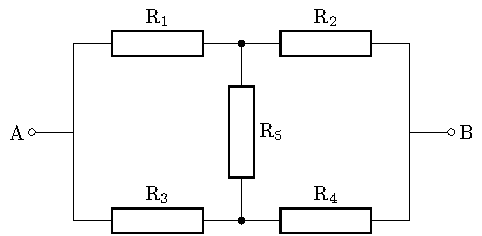
\includegraphics{q_circuit-extent_03_04/physics-standard_questions_circuit-extent_03_04_tikz.pdf}
        \par}
        \vspace{0.2\baselineskip}
    
    \item \needspace{8\baselineskip}
        図のように，12個の電気抵抗からなる回路がある．いずれの電気抵抗の抵抗値も$R$である．
        AB間の合成抵抗$R_\mathrm{AB}$を求めよ．
        \par \vspace{0.2\baselineskip}
        {\centering
            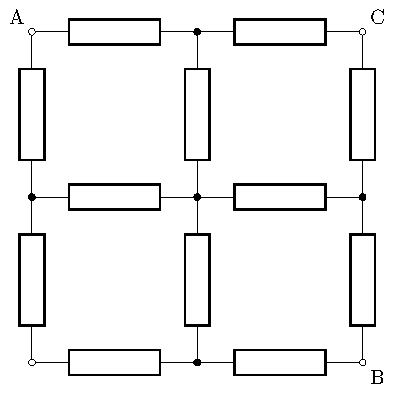
\includegraphics{q_circuit-extent_03_05/physics-standard_questions_circuit-extent_03_05_tikz.pdf}
        \par}
        \vspace{0.2\baselineskip}

\end{enumerate}

\end{document}
